\chapter{Monthly snapshots of the Internet AS-level network from BGP}

\resp{Giancarlo Venturato}

\section{Data and network reconstruction}

At the coarsest scale the Internet is a network of \emph{Autonomous Systems}
(ASes) that exchange reachability information through the Border Gateway
Protocol (BGP). We reconstruct one AS-level snapshot per month from the
routing-table dumps archived by the RIPE RIS collector
\texttt{rrc00}~\cite{ripeRIS}, taking the first available \texttt{bview} table
dump of each month (day~01 at 00:00~UTC when present; the exact file used is
recorded in a manifest). The archive spans \textbf{November 1999 -- April
2026}; 314 of the 318 calendar months yield a usable table (April--July 2000
are absent from the archive; in a few further months of 2000 and in June 2017
the first files are truncated, and the pipeline falls back to the largest
remaining dump of the month). Three formats occur and are all handled: modern
MRT \texttt{TABLE\_DUMP}/\texttt{TABLE\_DUMP\_V2} records, parsed with
\texttt{bgpdump}; the pre-2001 Zebra MRT dialect (many RIB entries packed into
one record, 16-bit ASNs); and the gzipped GateD \emph{text} tables of early
2000 --- the latter two read by purpose-written parsers validated against
neighbouring months.

Every \texttt{AS\_PATH} is cleaned as follows: consecutive duplicate ASNs are
collapsed (route prepending); malformed or empty paths are dropped; paths
containing \texttt{AS\_SET}s are dropped entirely, a documented simplification
affecting a median $0.02\%$ of entries per month; paths with fewer than two
ASNs are dropped. Overall $\geq 96.4\%$ of RIB entries are retained in every
month (median $99.9\%$; per-month statistics accompany the data). Each
consecutive ASN pair of a retained path becomes an undirected edge in
canonical $(\min,\max)$ order, self-loops are discarded, and the integer edge
weight counts the RIB entries in which the pair was observed that month;
ignoring the weight column yields the unweighted simple graph used for all
metrics below. ASNs are the integer AS numbers from the dumps, so node
identity is consistent across snapshots.

An essential caveat: these graphs are \emph{not} the physical Internet
topology but the AS-level topology \emph{as observed from a single collector}.
An edge is visible only if some BGP peer of \texttt{rrc00} propagates a route
through it, so peripheral (especially peer-to-peer) links are systematically
under-sampled and all counts are lower bounds~\cite{oliveira2010completeness}.
Moreover the collector's own peer set grows in time (the monthly table has
$4\times10^5$ RIB entries in 1999 and $5.5\times10^7$ in 2026), so part of any
temporal trend reflects improving \emph{visibility} rather than Internet
structure; we point out below where this matters.

\section{Growth and heavy-tailed connectivity}

Figure~\ref{fig:asgrowth} summarises 26.5 years of evolution: the visible AS
graph grows from $6\,045$ nodes and $10\,634$ edges (Nov.~1999) to $86\,114$
nodes and $239\,705$ edges (Apr.~2026) --- factors of $14.2$ and $22.5$
respectively. Edges outpace nodes, so the network densifies, but only mildly:
$\langle k\rangle$ rises from $3.5$ to $5.6$. The sharp $\langle k\rangle$
step around 2019--2021 coincides with a large expansion of the collector's
peer set and is largely a visibility effect, while the slow drift before it is
consistent with genuine densification of the AS ecosystem. The graph is one
connected component at all times (LCC $\geq 99.99\%$ of nodes in every
month), as expected for a routing-derived view.

The degree distribution is heavy-tailed in every snapshot
(Fig.~\ref{fig:asdegree}a), the classical signature of the AS
graph~\cite{faloutsos1999power}, with maximum degrees growing from
$\sim2.4\times10^3$ to $\sim1.1\times10^4$. Discrete maximum-likelihood
power-law fits~\cite{clauset2009power,alstott2014powerlaw} give a strikingly
stable exponent: $\hat\alpha$ stays within $[2.01, 2.21]$ for the whole
series (typical $\hat\sigma\approx0.03$), averaging $2.12$ in the first five
years and $2.10$ in the last five (Fig.~\ref{fig:asdegree}b) --- the
scale-free character of the AS topology is persistent while the network grows
by more than an order of magnitude. Following~\cite{clauset2009power} we also
compared power-law and lognormal fits of each snapshot: the log-likelihood
ratio mildly favours the lognormal in $282/314$ months but is statistically
inconclusive in $280$ of them ($p>0.1$), the well-known outcome that the AS
degree tail cannot be distinguished from a lognormal on data of this size ---
``power law'' is here a description of the regime
$P(k)\!\sim\!k^{-2.1}$ over $\sim$3 decades, not a model-selection claim.

\begin{figure}[H]
\centering
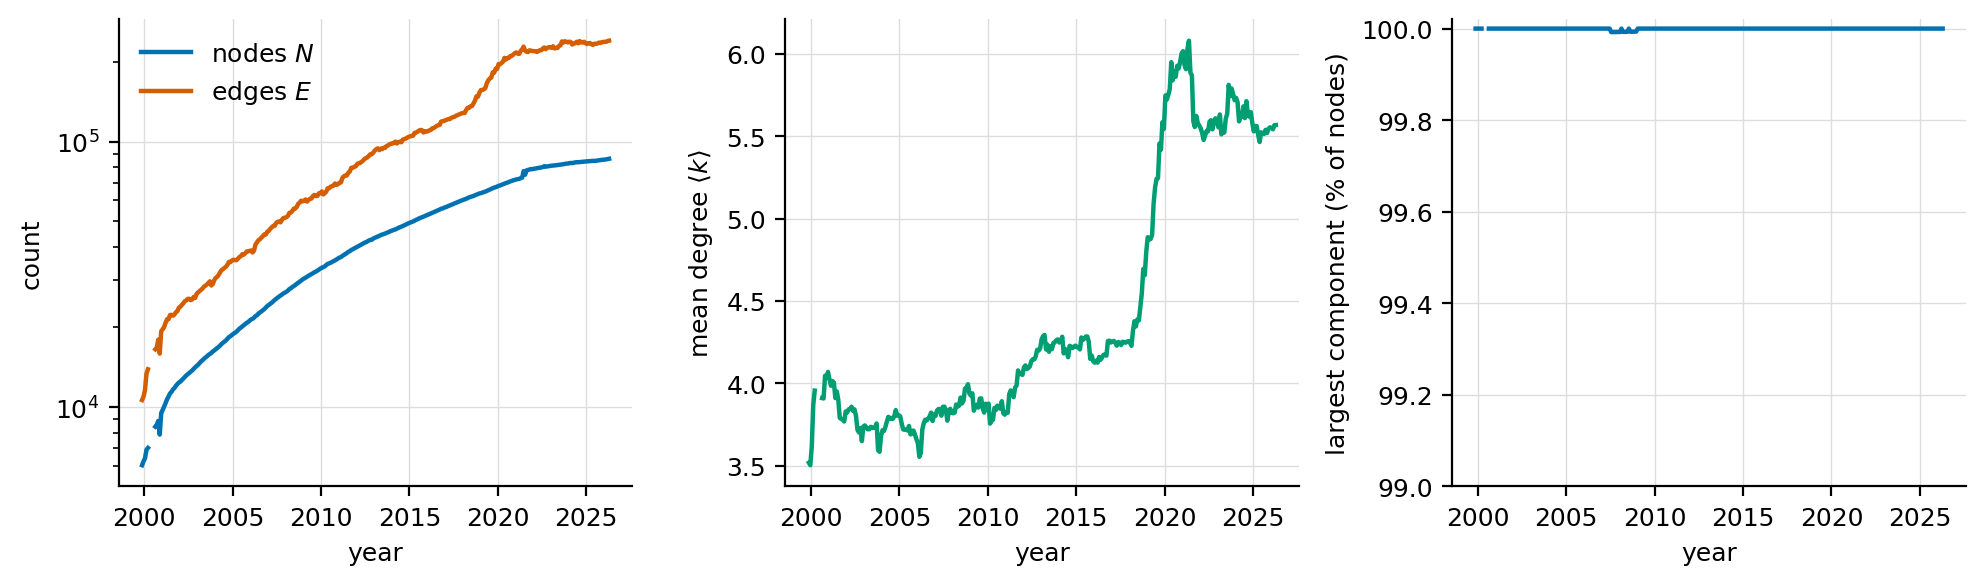
\includegraphics[width=\textwidth]{images/internet_fig1_growth.png}
\caption{Growth of the monthly AS graph, Nov.~1999 -- Apr.~2026. Node and edge
counts (left, log scale), mean degree (centre; the 2019--2021 step is largely
increased collector visibility), and largest-connected-component share
(right). Line breaks mark the Apr.--Jul.~2000 archive gap.}
\label{fig:asgrowth}
\end{figure}

\begin{figure}[H]
\centering
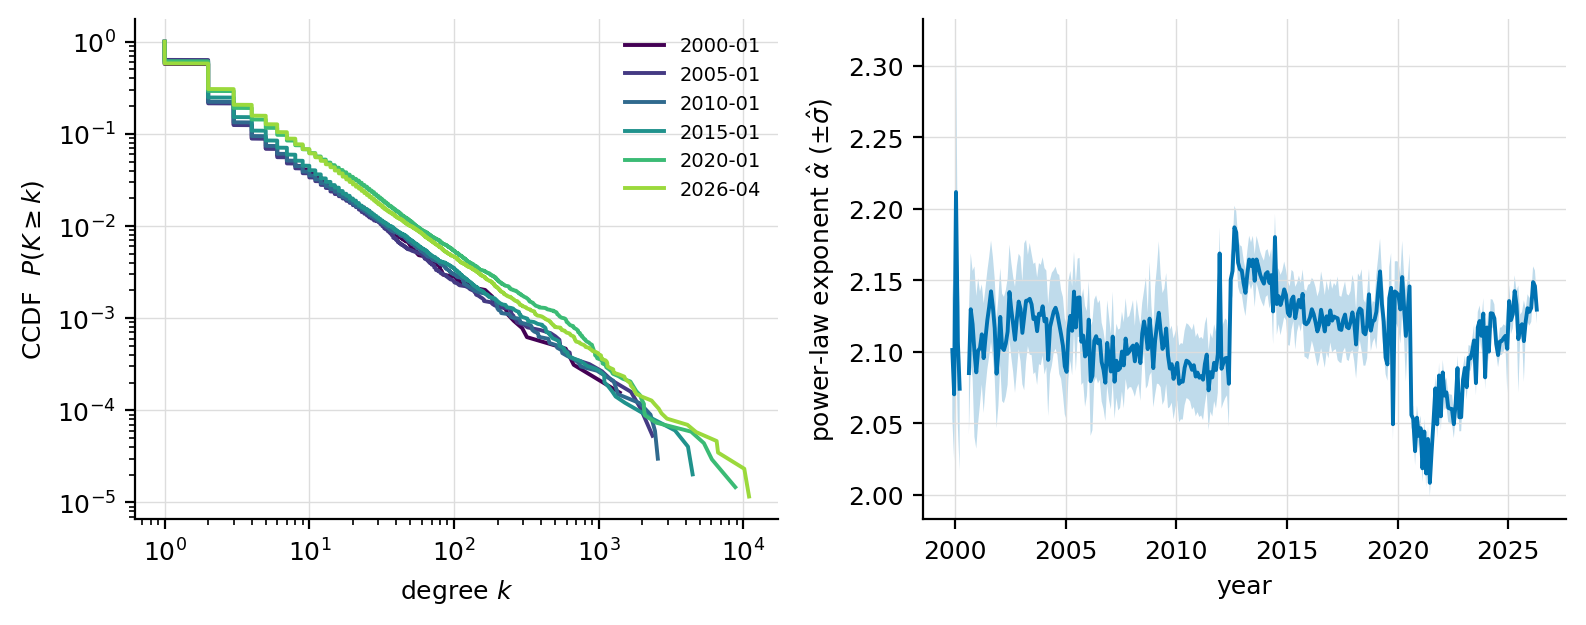
\includegraphics[width=0.9\textwidth]{images/internet_fig2_degree.png}
\caption{(a)~Degree CCDF of six snapshots spanning the series: the tail
$P(K\geq k)\sim k^{-1.1}$ ($\alpha\approx2.1$) simply extends to larger $k$ as
the network grows. (b)~Discrete MLE power-law exponent per month, with the
fitted $\pm\hat\sigma$ band.}
\label{fig:asdegree}
\end{figure}

\section{Turnover, correlations and communities}

Beneath the smooth aggregate growth the membership churns
(Fig.~\ref{fig:asturnover}): in a median month $1.3\%$ of ASes are new and
$0.7\%$ of the previous month's ASes disappear (node Jaccard overlap
$0.98$). Edges are far more volatile (Jaccard $0.90$), partly through genuine
rewiring of customer--provider relations and partly through fluctuating route
visibility; both rates decay over the years as the network matures. The apex
of the hierarchy, in contrast, is remarkably rigid: consecutive months share
$95\%$ of their top-20 highest-degree ASes on average, and hub identity
changes only on multi-year timescales --- the 1999 top of the list (AS701
UUNET, AS1239 Sprint, AS3561 Cable\,\&\,Wireless, AS7018 AT\&T) is gradually
replaced by AS174 (Cogent), AS3356 (Level\,3/Lumen) and, at the top since the
mid-2010s, AS6939 (Hurricane Electric). Hub \emph{identity} is sticky even as
hub degree grows by two orders of magnitude.

Degree--degree correlations are strongly disassortative throughout:
$\langle k_{nn}\rangle(k)\sim k^{\mu}$ (Fig.~\ref{fig:asstructure}a) with
$\mu\approx-0.53$ around 2000, the value reported for the early
Internet~\cite{pastorsatorras2001dynamical}. The exponent then drifts steadily
to $\mu\approx-0.70$ by 2024--2026 (Fig.~\ref{fig:asstructure}b): as the
periphery grows, low-degree customers hang ever more exclusively off
high-degree providers. Community structure found by Leiden modularity
optimisation~\cite{traag2019leiden} (Fig.~\ref{fig:asstructure}c,d) is
significant at all times but evolves: $Q$ rises to a plateau of
$\approx0.72$ around 2010, then falls to $\approx0.61$ after 2019 while the
number of communities triples ($\sim$30 to $\sim$80). The post-2019 drop
again partly tracks the visibility expansion --- more visible interconnection
(IXPs, content providers peering directly) genuinely flattens the hierarchy,
and a better-instrumented collector sees more of it.

\begin{figure}[H]
\centering
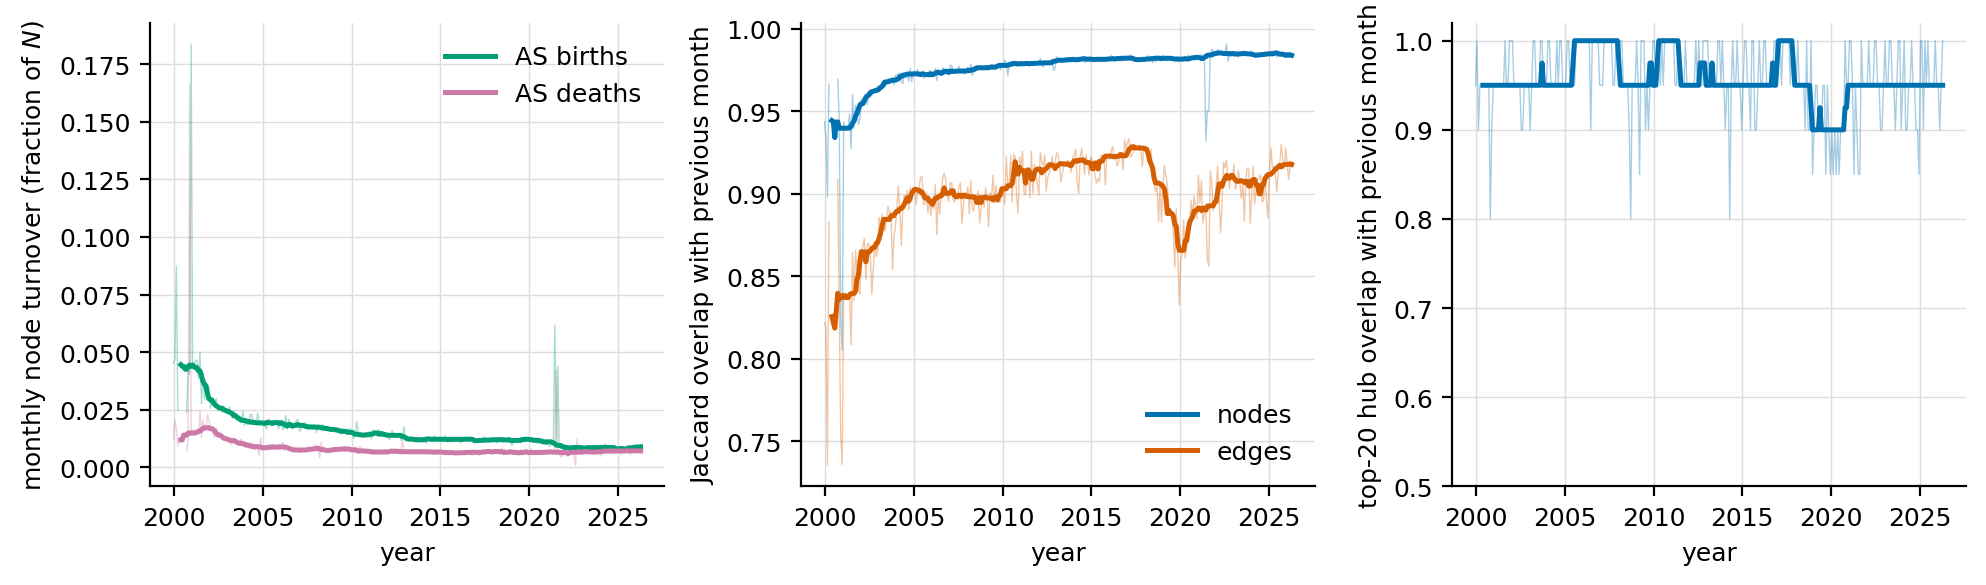
\includegraphics[width=\textwidth]{images/internet_fig3_turnover.png}
\caption{Monthly turnover (thin: raw; thick: 12-month rolling median).
(a)~AS birth/death rates. (b)~Node and edge Jaccard overlap between
consecutive months. (c)~Top-20 hub set overlap between consecutive months.}
\label{fig:asturnover}
\end{figure}

\begin{figure}[H]
\centering
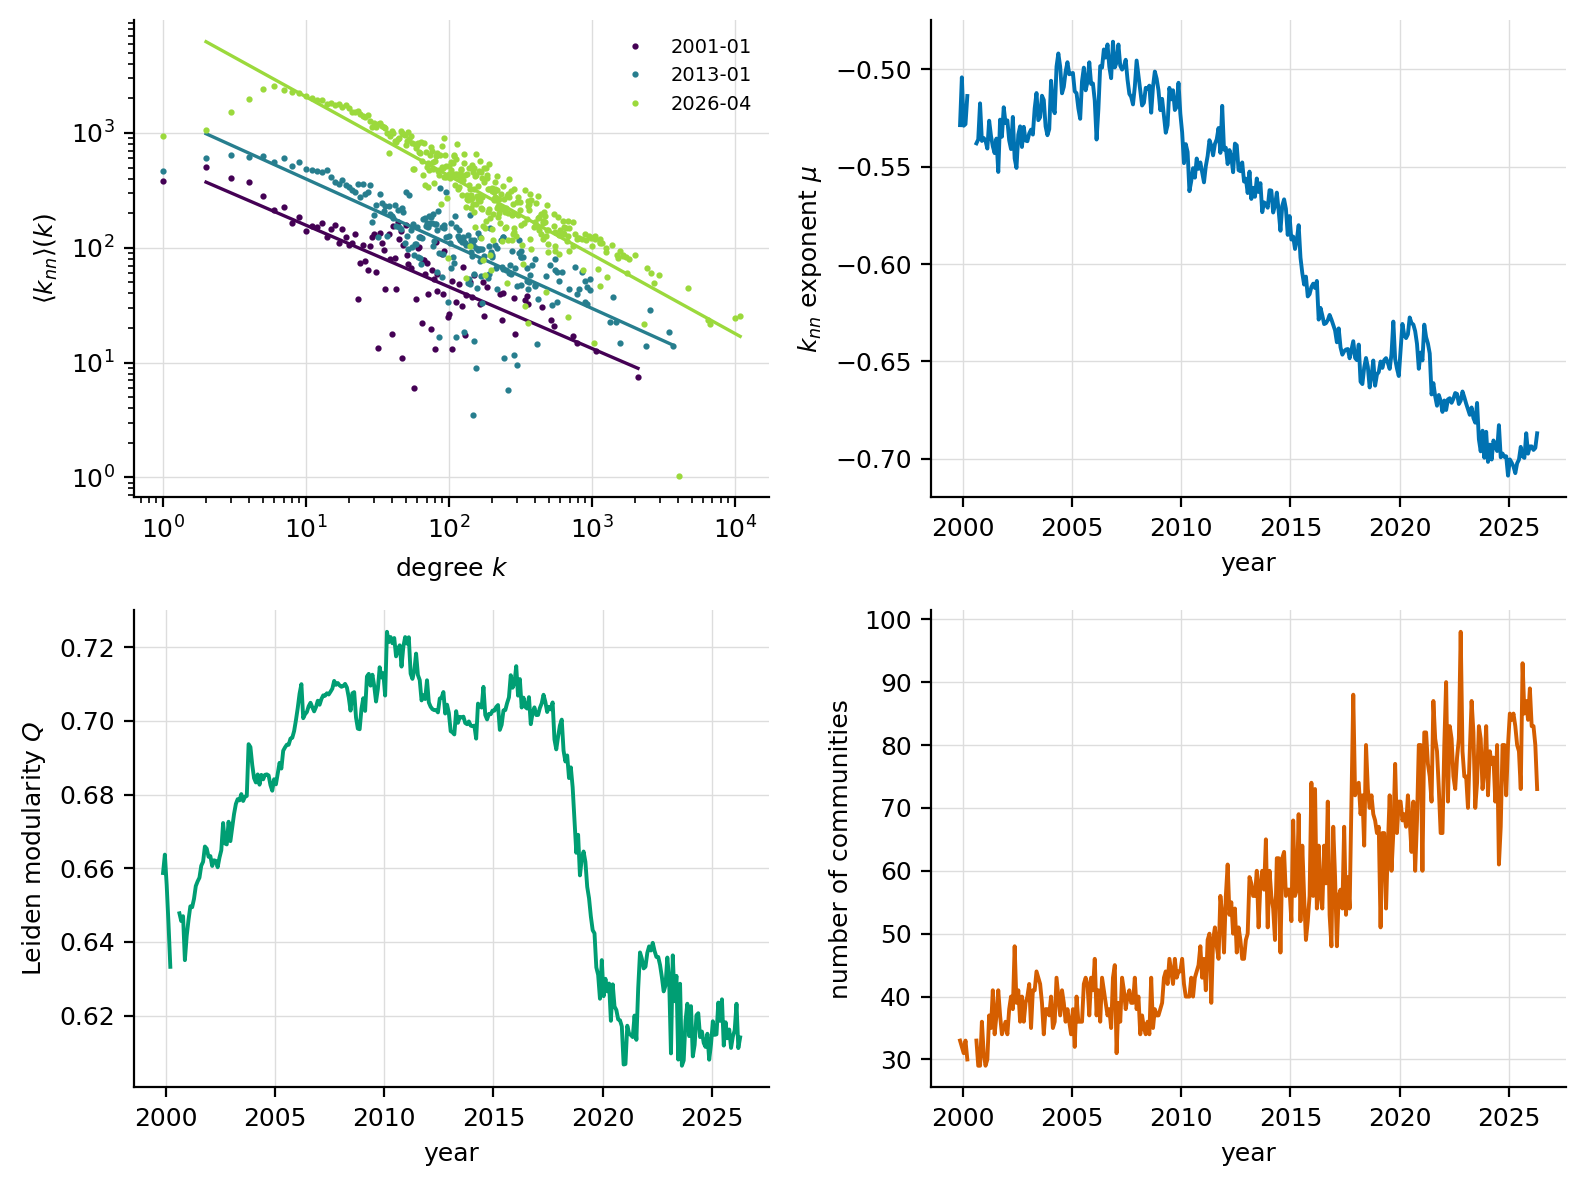
\includegraphics[width=0.92\textwidth]{images/internet_fig4_structure.png}
\caption{(a)~$\langle k_{nn}\rangle(k)$ for three snapshots with power-law
fits. (b)~Disassortativity exponent $\mu$ per month. (c)~Leiden modularity
and (d)~number of communities per month.}
\label{fig:asstructure}
\end{figure}
